\begin{figure}[H]
\centering
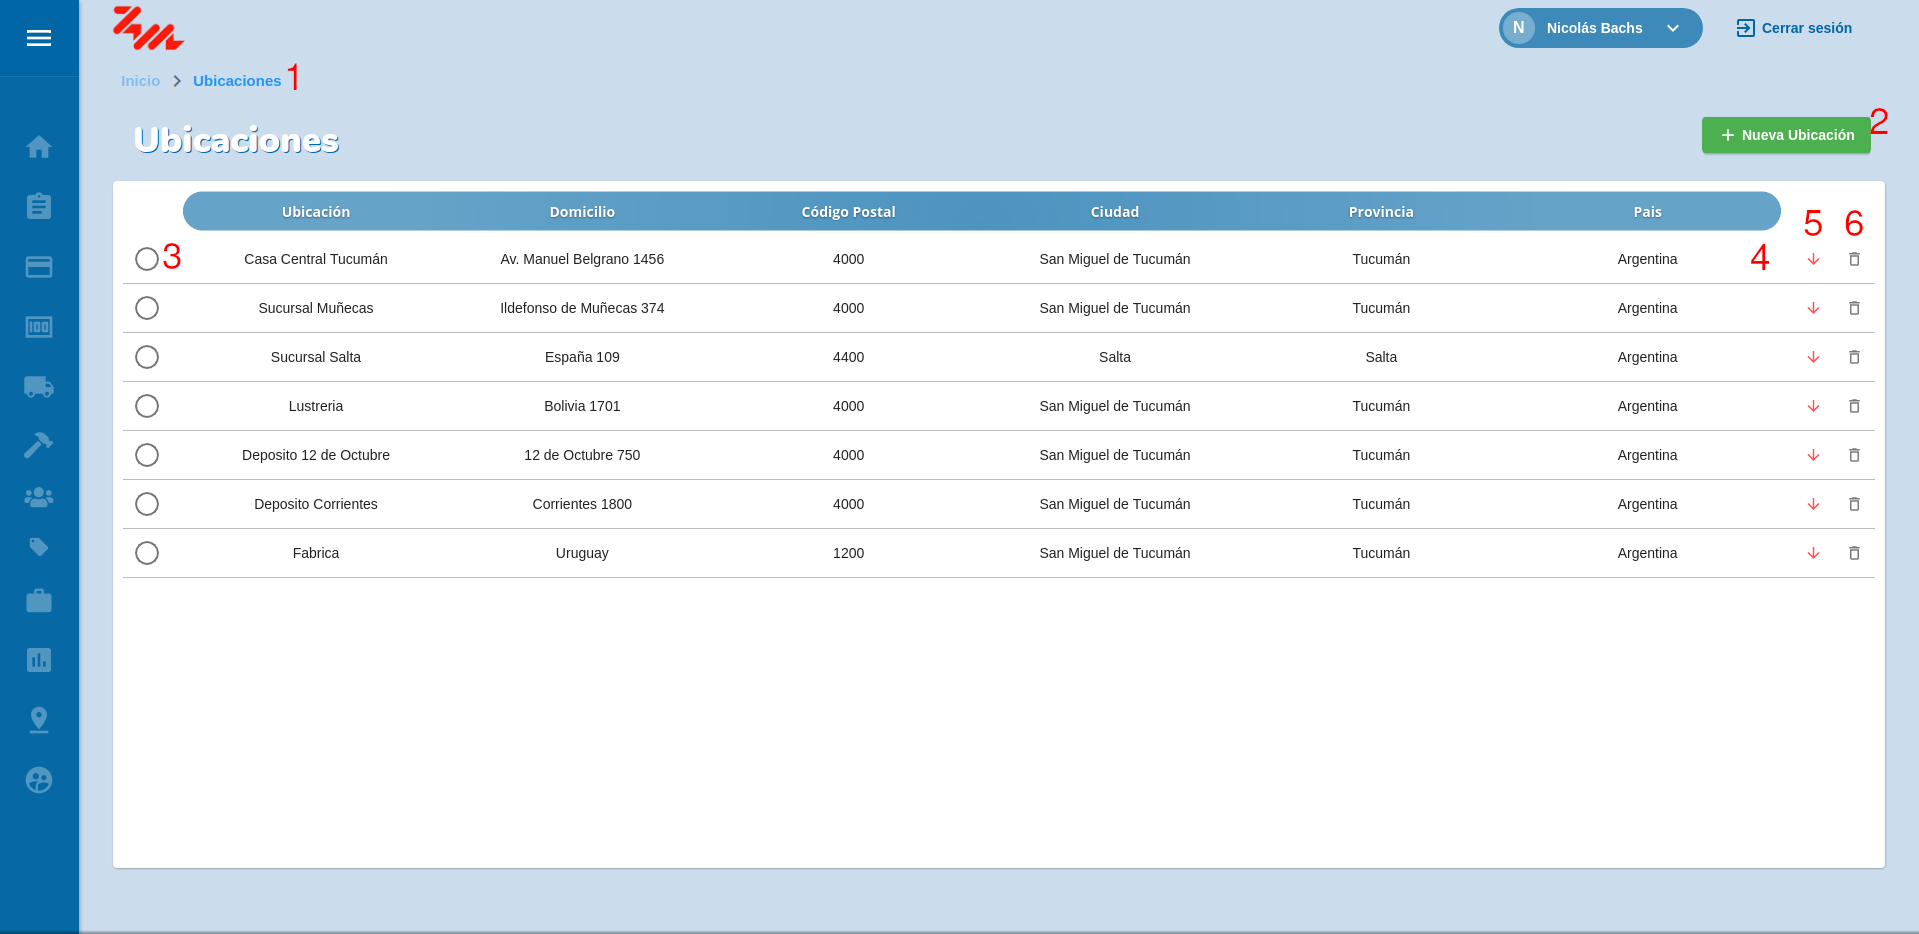
\includegraphics[width=\textwidth,height=\textheight,keepaspectratio]{Escenarios/AD-37-00}
\caption{Escenario - AD-37-00}
\label{fig:AD-37-00}
\end{figure}

Este escenario muestra toda la información referida a las ubicaciones, junto con las acciones disponibles.
El botón \textbf{AD-37-01} permite al usuario navegar al escenario \textbf{AD-02-00}. El botón \textbf{AD-37-02} permite al usuario crear una nueva ubicación y navega al escenario \textbf{AD-38-00}.
El botón \textbf{AD-37-03} permite al usuario seleccionar una o más ubicaciones del resultado de la búsqueda. Si existen ubicaciones seleccionados se mostrarán botones con las opción de borrar y activar/desactivar según corresponda. El campo \textbf{AD-37-04} muestra la información relacionada a las ubicaciones especificando su nombre, domicilio, código postal, ciudad, provincia y país. El botón \textbf{AD-37-05} permite al usuario dar de alta/baja una ubicación y el botón \textbf{AD-37-06} permite al usuario borrar la ubicación.
\clearpage
